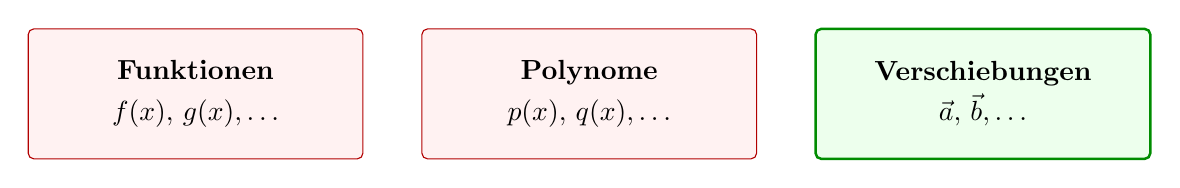
\begin{tikzpicture}[
  card/.style={
    draw=red!70!black,
    fill=red!5,
    rounded corners=2pt,
    minimum width=4.25cm,
    minimum height=1.65cm,
    align=center,
    inner sep=0.25cm
  },
  focus/.style={
    card,
    draw=green!55!black,
    fill=green!7,
    line width=0.9pt
  }
]
  \node[card] (functions) at (0,0)
    {\textbf{Funktionen}\\[0.25em]$f(x),\,g(x),\dots$};
  \node[card] (polynomials) at (5.0,0)
    {\textbf{Polynome}\\[0.25em]$p(x),\,q(x),\dots$};
  \node[focus] (translations) at (10.0,0)
    {\textbf{Verschiebungen}\\[0.25em]$\vec a,\,\vec b,\dots$};
\end{tikzpicture}
